%-------------------------------------------------
%	Version: 0.0
%	fecha de entrega 5 febrero 2021
%
%-------------------------------------------------

\documentclass[11pt]{report}

%packages
\usepackage{graphicx}
\usepackage{subcaption}

\usepackage[utf8]{inputenc}
\usepackage[spanish, es-nodecimaldot]{babel}
\usepackage{setspace}
\usepackage{ragged2e}

\usepackage{amsmath}
\usepackage{amsthm}
\usepackage{amssymb}
\usepackage{mathtools}
\usepackage{siunitx}
\usepackage[thinc]{esdiff} %derivadas faciles
\usepackage{physics} %algunos simbolos de derivadas

%path donde se encuentran las imagenes
\graphicspath{ {./figuras/} }

%---------------------------------------------------------------
%ABREVIACIONES DE COMANDOS
%---------------------------------------------------------------

\theoremstyle{plain}
\newtheorem{thm}{Teorema}[chapter] % reset theorem numbering for each chapter

\theoremstyle{definition}
\newtheorem{defn}[thm]{Definición} % definition numbers are dependent on theorem numbers
\newtheorem{exmp}[thm]{Ejemplo} % same for example numbers

\newcommand{\chaptercontent}{
\section{Basics}
\begin{defn}Here is a new definition.\end{defn}
\begin{thm}Here is a new theorem.\end{thm}
\begin{thm}Here is a new theorem.\end{thm}
\begin{exmp}Here is a good example.\end{exmp}
\subsection{Some tips}
\begin{defn}Here is a new definition.\end{defn}
\section{Advanced stuff}
\begin{defn}Here is a new definition.\end{defn}
\subsection{Warnings}
\begin{defn}Here is a new definition.\end{defn}
}

\usepackage{biblatex}
%\addbibresource{Tarea1.bib}

\begin{document}

\begin{titlepage}
\title{Ejercicios_notas}

%-------------------------------------------------
%PORTADA
%-------------------------------------------------

	\centering
	{\scshape\LARGE Universidad Autónoma de Yucatán  \\ Facultad de ingeniería\par}
	\vspace{1cm}
	{\scshape\Large Métodos matemáticos de la física\par}
	\vspace{1.5cm}
	{\huge\bfseries Ejercicios de las notas\par}
	\vspace{0.7cm}
	{\begin{figure}[!h]
	\centering
    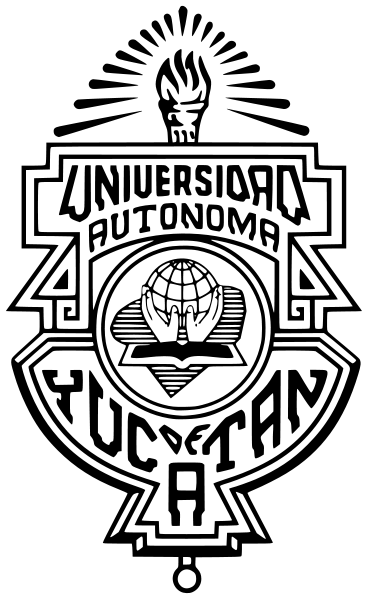
\includegraphics[scale=0.3]{UADY.png}
	\end{figure}}
	\vspace{0.7cm}
	{\Large\itshape Erick Al. Casanova Cortés\par}
	{\Large\itshape Matricula: 15014866\par}
	\vfill
	{\scshape\Large Docente\par
	Dr. Miguel Zambrano\par}
	\vfill
	{\Large{\bfseries Fecha de entrega: 5 Febrero 2021} }

	\vfill
	
\end{titlepage}

%-------------------------------------------------
%Inicio del documento
%-------------------------------------------------

\tableofcontents

%-------------------------------------------------
%Primer Ejercicio
%-------------------------------------------------
\part{Ejemplo 1}
\section{Definición del libro}

Desarrollar el ejemplo 2 de las notas de las transformadas de Fourier.\\
Ejemplo: Considera el oscilador armónico armortiguado que actúa en una fuerza externa $g(t)$. El movimiento del oscilador está situado por la ecuación:\\
\begin{equation*}
	\ddot{x}(t) + 2\alpha \dot x (t) + \omega^2_o x(t) = f(t)
\end{equation*}

donde $f(t) = \frac{1}{m} g(t)$\\

Por definición, podemos extender este resultado a:

\begin{align*}
	f(t) &= \int_{-\infty}^\infty \hat F(\omega) e^{i\omega t}\dd{\omega}\\
	f(t) &= \frac{1}{\sqrt{2\pi}}\int_{-\infty}^\infty \hat F(\omega) e^{-i\omega t} \dd{\omega}
\end{align*}

donde:

\begin{align*}
	\hat F(\omega)&=\frac{1}{2\pi}\int_{-\infty}^\infty f(t)e^{-i\omega t}\dd{t}\\
	\hat F(\omega) &= \frac{1}{\sqrt{2\pi}}\int_{-\infty}^\infty f(t)e^{i\omega t}\dd{t}
\end{align*}

Respectivamente\\

Esto conlleva a que la solución de $x$ también tendrá una transformada de Fourier que se denotará como $\hat A$, por lo que:

\begin{align*}
	x(t) &= \int_{-\infty}^\infty \hat A(\omega) e^{i\omega t}\dd{t}\\
	x(t) &= \frac{1}{\sqrt{2\pi}}\int_{-\infty}^\infty \hat A(\omega) e^{-i\omega t}\dd{t}
\end{align*}

Resulta evidente ver a $\hat A$ como la transformada de la ecuación diferencial, por lo que usando las propiedades de las derivadas de las transformadas obtenemos:

\begin{align*}
	\mathcal{F}\lbrace \dot{x} \rbrace &= -i\omega \mathcal{F}\lbrace x \rbrace\\
	\mathcal{F}\lbrace \ddot{x} \rbrace &= -\omega^2 \mathcal{F}\lbrace x \rbrace
\end{align*}

Con estas ecuaciones asumimos que $x(\pm \infty) = \dot x (\pm \infty) = 0$.\\
Por definición tenemos que:

\begin{align*}
	\int_{-\infty}^\infty \diff{}{t} x(t) e^{i\omega t} \dd{t}= -\int_{-\infty}^\infty x(t) \diff{}{t} e^{i\omega t} \dd{t}\\
\end{align*}

Por lo consiguiente, la transformada de la ecuación diferencial es:
\begin{equation*}
	-\omega^2 A(\omega) -2\alpha\omega iA(\omega)+\omega^2_oA(\omega) = F(\omega)
\end{equation*}

Despejando entonces $A(\omega)$

\begin{equation*}
	A(\omega) = \frac{F(\omega)}{(\omega^2_o -\omega)-2i\alpha\omega}
\end{equation*}

La solución al problema entonces es:

\begin{equation*}
	x(t)=\frac{1}{\sqrt{2\pi}}\int_{-\infty}^\infty \frac{F(\omega)e^{-i\omega t}}{\omega^2_o -\omega)-2i\alpha\omega}
\end{equation*}

Igualando el denominador a cero podemos ver que:

\begin{equation*}
	\omega^2_o -\omega)-2i\alpha\omega = \zeta (\omega)
\end{equation*}

\begin{align*}
	-\omega^2 -2i\alpha\omega + \omega^2_o &=0\\
	\omega &= \frac{2i\alpha \pm\sqrt{4\omega^2_o - 4\alpha^2}}{-2}\\
	\omega &= -i\alpha \pm \sqrt{-(\alpha^2-\omega^2_o)}
\end{align*}

Para los valores de $\alpha > 0$ los polos están arriba y se localizan en:

\begin{align*}
	\omega_{1, 2} &= \pm \sqrt{\omega^2_o -\alpha^2} -i\alpha & \text{Si $\omega_o>\alpha$}\\
	\omega_{1, 2} &= \pm i\sqrt{\alpha^2-\omega^2_o}-i\alpha & \text{Si $\omega_o<\alpha$}\\
	\omega_{1} &=\omega_{2} = -i\alpha & \text{Si $\omega_o=\alpha$}
\end{align*}

Ahora analizaremos los casos:\\
Pimer caso: Dos polos simples\\
Así tenemos que $\zeta(\omega) = -(\omega-\omega_1)(\omega-\omega_2)$, por lo que al evaluar los residuos obtenemos en $\omega = \omega_1$:

\begin{equation*}
	\frac{1}{\sqrt{2\pi}}\frac{F(\omega_1)e^{-i\omega_1t}}{\omega_1 - \omega_2}
\end{equation*}

Y cuando tenemos el caso de $\omega = \omega_2$:

\begin{equation*}
	-\frac{1}{\sqrt{2\pi}}\frac{F(\omega_2)e^{-i\omega_2t}}{\omega_1 - \omega_2}
\end{equation*}

Donde $\omega_1-\omega_2 = 2\sqrt{\omega^2_0 -\alpha^2}=2p$\\

Como ejemplo particular, asumir que $f(t)$ tiene la forma

\begin{equation*}
	f(t)=
	\begin{cases}
		fo & |t|<\tau\\
		0 & |t|\geq\tau
	\end{cases}
\end{equation*}

La transformada de Fourier de $f(t)$:
\begin{align*}
	F(\omega)&=\frac{f_o}{\sqrt{2\pi}}\int_\tau^\tau e^-{i\omega t}\dd{t}\\
	&=f_o\sqrt{\frac{2}{\pi}}\frac{\sin 	\omega\tau}{\omega}
\end{align*}

Entonces es evidente que:

\begin{equation*}
	x(t)=-\frac{f_o}{\pi}\int_{-\infty}^\infty \frac{\sin\omega\tau e^{-i\omega\tau}}{\omega(\omega-\omega_1)(\omega-\omega_2)}\dd{\omega}
\end{equation*}

donde $\omega_1=\sqrt{\omega^2_o -\alpha^2}-i\alpha$, $\omega_2=-\sqrt{\omega^2_o -\alpha^2}-i\alpha$. Las únicas singularidades son en $\omega=\omega_1$, $\omega=\omega_2$.

\begin{equation*}
	\sin\omega\tau = \frac{1}{2}(e^{i\omega\tau}-e^{-i\omega\tau})
\end{equation*}

Entonces $t>\tau$, la función $\frac{\sin\omega\tau e^{-i\omega\tau}}{\omega}$ está encerrada.

Esto da entonces que:

\begin{equation*}
	x(t)=\frac{2i\pi f_o}{\pi} \lbrack \frac{ \sin\omega_{1}\tau e^{-i\omega_1\tau} }{\omega_1(\omega_1-\omega_2)} -\frac{ \sin\omega_{2}\tau e^{-i\omega_2\tau} }{\omega_2(\omega_1-\omega_2}\rbrack
\end{equation*}

\begin{equation*}
	x(t)=\frac{2if_o}{\omega_1 \omega_2(\omega_1-\omega_2}(\omega_2\sin\omega_{1}\tau e^{-i\omega_1\tau} - \omega_2\sin\omega_{2}\tau e^{-i\omega_2\tau})
\end{equation*}

Para una forma real hay que hacer que  $\omega_1 =\sqrt{\omega^2_o -\alpha^2}-i\alpha$, $\omega_2=-\sqrt{\omega^2_o -\alpha^2}-i\alpha$; $\omega_1\omega_2 = -\omega^2_o$ y expresar el seno en términos del exponencial:

\begin{align*}
	x(t)&=\frac{2i\pi f_o}{\pi}(e^{(\alpha+ip)(\tau-t)} + (e^{(\alpha-ip)(\tau-t)} - e^{-(\alpha+ip)(\tau-t)} - (e^{-(\alpha-ip)(\tau-t)}\\
	&+(\frac{i\alpha}{p})(e^{(\alpha+ip)(\tau-t)} - (e^{(\alpha-ip)(\tau-t)} - e^{-(\alpha+ip)(\tau-t)} - (e^{-(\alpha-ip)(\tau-t)} ))
\end{align*}

Lo que es igual a


\begin{align*}
	x(t)&=\frac{2i\pi f_o}{\pi}\lbrack\cos p(t-\tau) + (\frac{i\alpha}{p})\sin p(t-\tau)\rbrack e^{-\alpha(t-\tau)}\\ 
	&- \frac{2i\pi f_o}{\pi}\lbrack \cos p(t-\tau) + \frac{\alpha}{p}\sin(t-\tau)\rbrack e^{-\alpha(t-\tau)}
\end{align*}

Para $t<-\tau$ el contorno cierra arriba y será cero
%-------------------------------------------------
%Segundo ejercicio
%-------------------------------------------------
\part{Ejemplo 1}
\section{Definición vista en clase}

Desarrollar el ejemplo 2 de las notas de las transformadas de Fourier.\\
Ejemplo: Considerar el oscilador armónico amortiguado que actúa en una fuerza externa $g(t)$. El movimiento del oscilador está situado por la ecuación:
\begin{equation*}
	\ddot{x}(t) + 2\alpha \dot x (t) + \omega^2_o x(t) = f(t)
\end{equation*}

donde $f(t) = \frac{1}{m} g(t)$\\

Por definición, podemos extender este resultado a:

\begin{align*}
	f(t) &= \frac{1}{\sqrt{2\pi}}\int_{-\infty}^\infty \hat F(\omega) e^{i\omega t}\dd{\omega}\\
	f(t) &= \int_{-\infty}^\infty \hat F(\omega) e^{-i\omega t} \dd{\omega}
\end{align*}

Para este caso en específico utilzaremos:

\begin{align*}
	x(t) &= \frac{1}{\sqrt{2\pi}}\int_{-\infty}^\infty \hat A(\omega) e^{-i\omega t}\dd{t}
\end{align*}

Resulta evidente ver a $\hat A$ como la transformada de la ecuación diferencial, por lo que usando las propiedades de las derivadas de las transformadas obtenemos:

\begin{align*}
	\mathcal{F}\lbrace \dot{x} \rbrace &= -i\omega \mathcal{F}\lbrace x \rbrace\\
	\mathcal{F}\lbrace \ddot{x} \rbrace &= -\omega^2 \mathcal{F}\lbrace x \rbrace
\end{align*}

Sustituyendo en la ecuación diferencial:

\begin{equation*}
	-\omega^2 A(\omega) -2\alpha\omega iA(\omega)+\omega^2_oA(\omega) = F(\omega)
\end{equation*}

Despejando entonces $A(\omega)$

\begin{equation*}
	A(\omega) = \frac{F(\omega)}{(\omega^2_o -\omega)-2i\alpha\omega}
\end{equation*}
%--
\begin{equation*}
	x(t)=\frac{1}{\sqrt{2\pi}}\int_{-\infty}^\infty \frac{F(\omega)e^{-i\omega t}}{\omega^2_o -\omega)-2i\alpha\omega}
\end{equation*}

Igualando el denominador a cero podemos ver que:

\begin{equation*}
	\omega^2_o -\omega)-2i\alpha\omega = \zeta (\omega)
\end{equation*}

\begin{align*}
	-\omega^2 -2i\alpha\omega + \omega^2_o &=0\\
	\omega &= -\frac{2i\alpha \pm\sqrt{4\omega^2_o - 4\alpha^2}}{-2}\\
	\omega &= -i\alpha \pm \sqrt{-(\alpha^2-\omega^2_o)}
\end{align*}

Si los valores de $\alpha>0$ quiere decir que los polos se localizan en:

% casos de \omeega?
\begin{equation*}
	\omega_{1,2} = \pm \sqrt{\omega^2_o-\alpha^2}+i\alpha \text{ Si $\omega_o > \alpha$}
\end{equation*}

\begin{equation*}
	\omega_{1,2} = \pm i\sqrt{\omega^2_o-\alpha^2}+i\alpha \text{ Si $\omega_o < \alpha$}
\end{equation*}

\begin{equation*}
	\omega_{1} = \omega_{2} = i\alpha \text{ doble raiz en $\omega_o = \alpha$}
\end{equation*}

Analizando el caso de dos polos simples:\\
En este caso tenemos que $\zeta(\omega) = -(\omega - \omega_1)(\omega-\omega_2)$, evaluando los residuos tenemos que:
En $\omega = \omega_1$

\begin{equation*}
	\frac{\hat F (\omega_1) e^{i\omega_1 t}}{\omega_1-\omega_2}
\end{equation*}

En $\omega = \omega_2$

\begin{equation*}
	-\frac{\hat F (\omega_2) e^{i\omega_1 t}}{\omega_1-\omega_2}
\end{equation*}

Donde $\omega_1 - \omega_2 = 2\sqrt{\omega^2_o -\alpha^2} = 2\gamma$.

Consideramos al función de la forma:

\begin{equation*}
	f(t)=
	\begin{cases}
		fo & |t|<\tau\\
		0 & |t|>\tau
	\end{cases}
\end{equation*}

La transformada de Fourier de $F(t)$

\begin{align*}
	\hat F(\omega) &= f_o \int^\infty_{-\infty} e^{-i\omega t} \dd{t}\\
	&= \frac{2f_o}{2}\frac{1}{-i\omega}e^{-i\omega t}|^\tau_{-\tau}\\
	&= -\frac{f_o}{\pi\omega}\frac{e^{-i\omega \tau}- e^{-i\omega \tau}}{2i}\\
	&= \frac{2f_o\sin\omega\tau}{\omega}
\end{align*}

Entonces las soluciones quedan:

\begin{equation*}
	x(t)=\frac{2f_o}{2\pi}\int^\infty_{-\infty} \frac{\sin(\omega\tau) e^{i\omega t}}{\omega(\omega-\omega_1)(\omega	-\omega_2)}\dd{\omega}
\end{equation*}

Se emplea el teorema del residuo y se observa que los polos se encuentran:

\begin{align*}
	x(t)=\frac{2i\pi f_o}{\pi}(\frac{\sin(\omega_2\tau) e^{i\omega_2 t}}{\omega_2(\omega_1-\omega_2)}-\frac{\sin(\omega_1\tau) e^{i\omega_1 t}}{\omega_1(\omega_1-\omega_2)})
\end{align*}

Así queda entonces:
\begin{align*}
	x(t)=\frac{2if_o}{\omega_1\omega_2(\omega_1-\omega_2)}(
	\sin(\omega_2\tau) e^{i\omega_2 t} - \sin(\omega_1\tau) e^{i\omega_1 t})
\end{align*}

Para obtener una forma real proponemos entonces $\omega_1 = \gamma + i\alpha$, $\omega_2 = -\gamma + i\alpha$\\

\begin{equation*}
	\omega_1\omega_2 = -\omega^2_o
\end{equation*}

\begin{equation*}
	\omega_1-\omega_2 = 2\gamma
\end{equation*}

\begin{align*}
	x(t)&=\frac{fo}{-\omega^2_o} ((\gamma +i\alpha)(\frac{e^{2-(\gamma+i\alpha)\tau}-e^{-i(-\gamma+i\alpha)\tau}}{2}) e^{i(-\gamma+i\alpha)\tau}\\
	&-(-\gamma +i\alpha)(\frac{e^{i(\gamma+i\alpha)\tau}-e^{-i(\gamma+i\alpha)\tau}}{2}) e^{i(\gamma+i\alpha)\tau}
\end{align*}

\begin{align*}
	x(t)&= \frac{f_0}{2\omega_o^2\gamma} \lbrace (-\gamma +i\alpha) (e^{i(\gamma+i\alpha)\tau} - e^{-i(\gamma +i\alpha)\tau}) e^{i(-\gamma+i\alpha)\tau}\\ 
	&- (\gamma +i\alpha) (e^{i(\gamma+i\alpha)\tau} - e^{-i(-\gamma +i\alpha)\tau}) e^{i(-\gamma+i\alpha)\tau}\rbrace\\
	x(t)&= \frac{f_0}{2\omega_o^2}\lbrace -e^{-\alpha+i\gamma)(\tau+t)}+e^{(-\alpha+i\gamma)(t-\tau)}-e^{-\alpha-i\gamma)(\tau+t)}+e^{(-\alpha-i\gamma)(t-\tau)}\\
	&+(\frac{i\alpha}{\gamma})(e^{-\alpha+i\gamma)(\tau+t)}-e^{(-\alpha+i\gamma)(t-\tau)}-e^{-\alpha-i\gamma)(\tau+t)}+e^{(-\alpha-i\gamma)(t-\tau)})\rbrace\\
	x(t)&= \frac{f_0}{2\omega_o^2}\lbrace\cos(\gamma(t-\tau))+\frac{\alpha}{\gamma}\sin(\gamma(t-\tau))\rbrace e^{-\alpha(t-\tau)}\\
	&- \frac{f_0}{2\omega_o^2}\lbrace\cos(\gamma(t+\tau))+\frac{\alpha}{\gamma} \sin(\gamma(t+\tau))\rbrace e^{-\alpha(t+\tau)}
\end{align*}

%-------------------------------------------------
%Tercer ejercicio
%-------------------------------------------------
\part{Tarea 1 Ecuaciones diferenciales parciles}
%--- primer ejercicio
\section{Primer ejercicio}
A stretched string of length $L$ is "plucked" at the point and it's initial shape is given by:\\

\begin{equation*}
	\mu(x,o) = 
	\begin{cases}
		\frac{hx}{\varepsilon} & x<\varepsilon\\
		\frac{h(l-x)}{L-\varepsilon} & x\leq\varepsilon\\
	\end{cases}
\end{equation*}

The initial distribution of velocities is zero, that is $\pdv{t}\mu(x,o)=0$. Show that the motion of the string is given by the equation:\\

\begin{equation*}
	\mu(x,t)=\frac{2h^2}{\pi^L\varepsilon(L-\varepsilon)}\sum^\infty_{n=1}\frac{1}{\pi^2}\sin(\frac{n\pi\varepsilon}{L})\sin(\frac{n\pi x}{L})\cos(\frac{n\pi ct}{L})
\end{equation*}

La solución general está dada por:
\begin{equation*}
	\mu(x,t)=\sum^\infty_{n=1}\lbrace An\cos(\frac{n\pi ct}{L}) + Bn\sin(\frac{n\pi ct}{L})\rbrace\sin(\frac{n\pi x}{L})
\end{equation*}
Las condiciones iniciales $\pdv{\mu(x,t)}{t}=V_o(x)=0$

\begin{equation*}
	\pdv{\mu(x,t)}{t}=Bn\frac{cn\pi}{L}\sin(\frac{xn\pi}{L})
\end{equation*}
Por lo que $Bn=0$ para cualquier $n$. Por lo tanto, obtenemos de la segunda condición inicial:

\begin{equation*}
	\mu(x,0)=\sum^\infty_{n=1}An\sin(\frac{xn\pi}{L})
\end{equation*}

o

\begin{equation*}
	\mu(x,0)=An\sin(\frac{xn\pi}{L})
\end{equation*}

Entonces necesitamos encontrar el coeficiente $An$, el cual obtenemos al transformar $\mu(x,0)$ a una serie seno de Fourier:

\begin{equation*}
	An=\frac{1}{L}\int^L_0\mu(x,0)\sin(\frac{nx\pi}{L})\dd{x}
\end{equation*}

\begin{equation*}
	An=\frac{1}{L} \lbrace\int^\varepsilon_0 x\sin(\frac{nx\pi}{L})\dd{x} + \frac{h}{L-\varepsilon}\int^L_\varepsilon x\sin(\frac{nx\pi}{L})\dd{x}\rbrace
\end{equation*}

\begin{equation*}
	\int x\sin(\frac{nx\pi}{L})\dd{x} = -\frac{Lx}{n\pi}x\cos(\frac{nx\pi}{L}) + \frac{L^2}{n^2\pi^2}\sin(\frac{nx\pi}{L}) 
\end{equation*}

\begin{align*}
	An &=\frac{1}{L} \lbrace -\frac{Lx}{n\pi}x\cos(\frac{nx\pi}{L}) + \frac{L^2}{n^2\pi^2}\sin(\frac{nx\pi}{L})\rbrace^\varepsilon_0 \\
	&+ \frac{h}{L-\varepsilon}\lbrace\sin(\frac{nx\pi}{L})\rbrace^L_\varepsilon \\
	&- \frac{h}{L-\varepsilon}\lbrace -\frac{Lx}{n\pi}\cos(\frac{nx\pi}{L}) + \frac{L^2}{n^2\pi^2}\sin(\frac{nx\pi}{L})\rbrace^L_\varepsilon
\end{align*}

\begin{align*}
	An &= \frac{2}{L}(-\frac{Lh}{n\pi}\cos(\frac{n\pi\varepsilon}{L}) + \frac{L^2h}{n^2\pi^2\varepsilon}\sin(\frac{n\pi\varepsilon}{L}) + \frac{L^2h}{n^2\pi^2(L-\varepsilon)}\cos(\frac{n\pi\varepsilon}{L}) \\
	&- \frac{Lh\varepsilon}{n\pi(L-\varepsilon)}\cos(\frac{n\pi\varepsilon}{L}) +\frac{L^2h}{n^2\pi^2(L-\varepsilon)}\sin(\frac{n\pi\varepsilon}{L}))
\end{align*}

\begin{align*}
	\frac{2h}{n^2\pi^2}\left(\frac{L\sin(\frac{n\pi\varepsilon}{L})-n\pi\varepsilon\cos(\frac{n\pi\varepsilon}{L})}{\varepsilon} + \frac{L\sin(\frac{n\pi\varepsilon}{L})+n\pi(L-\varepsilon)\cos(\frac{n\pi\varepsilon}{L})}{L-\varepsilon}\right)
\end{align*}

\begin{align*}
	An = \frac{2hL^2}{\pi^2\varepsilon(L-\varepsilon)n^2}\sin(\frac{n\pi\varepsilon}{L})
\end{align*}

Finalmente con $Bn=0$

\begin{equation*}
	\mu(x,t)=\frac{2hL^2}{\pi^2\varepsilon(L-\varepsilon)}\sum^\infty_{n=1}\frac{1}{n^2}\sin(\frac{n\pi\varepsilon}{L})\sin(\frac{n\pi x}{L})\cos(\frac{n\pi ct}{L})
\end{equation*}


%- segundo ejercicio
\section{Segundo ejercicio}
When a piano string of lenght L is stuck by the piano hammer near the point $x=\varepsilon$, it's assumed that the inicial distribution of velocities is given by:

\begin{equation*}
	v_o(x)=
	\begin{cases}
		v_o\cos(\frac{\pi (x-\varepsilon)}{d}) & \text{para }|x-\varepsilon | < \frac{a}{2}\\
		0 & \text{para }|x-\varepsilon | > \frac{a}{2}
	\end{cases}
\end{equation*}

Asumimos que no hay un desplazamiento inicial y que el movimiento está dado por:

\begin{equation*}
	\mu(x,t)=\frac{4v_oD}{\pi^2 c}\sum^\infty_{n=1} \frac{1}{n}\frac{\sin(\frac{n\pi\varepsilon}{L})\cos(\frac{n\pi\varepsilon}{2L})}{1-\frac{n^2d^2}{L^2}}\sin(\frac{n\pi x}{L})\cos(\frac{n\pi ct}{L})
\end{equation*}

La solución general de la ecuación diferencial se puede expresar como:
\begin{equation*}
	\mu(x,t)=\sum^\infty_{n=1}\lbrace An\cos(\frac{n\pi ct}{L}) + Bn\sin(\frac{n\pi ct}{L})\rbrace\sin(\frac{n\pi x}{L})
\end{equation*}

Para las condiciones iniciales de $\mu(x,0) = 0$ podemos ver que:
\begin{align*}
	\mu(x,0) = An\sin(\frac{n\pi x}{L})
\end{align*}

Lo cual es igual a cero, lo que nos dice que $An = 0$, por lo tanto la solución queda expresada solo en términos de $Bn$, entonces expandiendo a $v_o$ en la serie senos de Fourier obtenemos:

\begin{align*}
	Bn = \frac{L}{cn\pi}\frac{2}{L}\int^L_0 v_o(x)\sin(\frac{n\pi x}{L})\dd{x}
\end{align*}

\begin{align*}
	Bn = \frac{2}{cn\pi}\int^{\varepsilon}_{	\varepsilon} v_o(x)\cos(\frac{\pi (x-\varepsilon)}{d})\sin(\frac{n\pi x}{L})\dd{x}
\end{align*}

Al resolver la integral podemos ver que:

\begin{align*}
	Bn = \frac{4v_od}{c\pi^2n}\frac{\sin(\frac{n\pi\varepsilon}{L})\cos(\frac{n\pi d}{2L})}{1-\frac{d^2n^2}{L^2}}
\end{align*}

Regresando a la función inicial vemos que:

\begin{equation*}
	\mu(x,t)=\sum^\infty_{n=1}\lbrace \frac{4v_od}{c\pi^2n}\frac{\sin(\frac{n\pi\varepsilon}{L})\cos(\frac{n\pi d}{2L})}{1-\frac{d^2n^2}{L^2}} \sin(\frac{n\pi ct}{L})\rbrace\sin(\frac{n\pi x}{L})
\end{equation*}

%-------------------------------------------------
%Cuarto ejercicio
%-------------------------------------------------
\part{Tarea 2}
\section{Primer ejercicio}
Demostrar que $\mathcal{J}_{-1/2}(x) = \sqrt{\frac{2}{x\pi}}\cos(x)$

\begin{align*}
	\mathcal{J}_{-1/2}(x) = \left(\frac{x}{2}\right)^{-1/2} \sum^\infty_{k=0} \frac{(-1)^k}{k!\pi(k+1/2)} \left(\frac{x}{2}\right)^{2k}
\end{align*}

\section{Segundo ejercicio}
Demostrar que las funciones $\mathcal{J}_{1/2}(x)$ y $\mathcal{J}_{-1/2}(x)$ son soluciones de la ecuación diferencia:

\begin{equation*}
	x^2y'' + xy' + (x^2 - 1/4)y=0
\end{equation*}
%-------------------------------------------------
%Final del documento
%-------------------------------------------------

\end{document}
